\documentclass[journal]{IEEEtran}

\usepackage{amsmath,cite,graphicx}

\begin{document}

\title{The Constant-Q Transform Spectral Envelope Coefficients: A Timbre Feature Designed for Music}

\maketitle

\section{Scope}

\IEEEPARstart{T}{imbre} is the attribute of sound which makes, for example, two musical instruments playing the same note sound different. It is generally associated with the spectral (but also temporal) envelope and is typically assumed to be independent from the pitch (but also the loudness) of the sound \cite{moore2004}. In this article, we will show how to design a simple but functional pitch-independent timbre feature which is well-adapted to musical data, by deriving it from the constant-Q transform (CQT) \cite{brown1991, brown1992}, a log-frequency transform which matches the equal temperament musical scale. We will show how to decompose the CQT-spectrum into an energy-normalized pitch component and a pitch-independent spectral envelope, the latter from which we will extract a number of timbral coefficients. We will then evaluate the discriminative power of these CQT-spectral envelope coefficients (CQT-SEC) on the NSynth dataset \cite{engel2017}, a large-scale dataset of musical notes which is publicly available, comparing them with the mel-frequency cepstral coefficients (MFCCs) \cite{mermelstein1976}, features originally designed for speech recognition but commonly used to characterize timbre in music. 


\section{Relevance}

A timbre feature which is well-adapted to musical data, pitch-independent, and with high discriminative power can find uses in a number of applications, such as similarity detection, sound recognition, and audio classification, in particular, of musical instruments. Additionally, the ability to decompose the spectrum of a sound (here, the CQT-spectrum) into a pitch-independent spectral envelope and an energy-normalized pitch component can be useful for analysis, transformation, and resynthesis of music signals. The energy-normalized pitch component can also potentially be used for tasks such as pitch identification, melody extraction, and chord recognition.


\section{Prerequisites}

Basic knowledge of audio signal processing and some knowledge of music information retrieval (MIR) \cite{mueller2007} are required to understand this article, in particular, concepts such as the Fourier transform (FT), convolution, spectral envelope, pitch, CQT, and MFCCs. More information about the CQT can also be found in \cite{brown1991, brown1992}.


\section{Problem Statement}

The multidimensional nature of timbre makes it an attribute that is tricky to quantify in terms of one simple characteristic feature \cite{grey1977}. While it is assumed to be independent from pitch and loudness, it is not really feasible to fully disentangle timbre from those qualities, as timbre is inherently dependent on the spectral content of the sound, which is also defined by its pitch and loudness \cite{moore2004}. Researchers in MIR proposed a number of descriptors to characterize one or more aspects of timbre \cite{peeters2011}, but they mostly resort to using the MFCCs when they need one simple timbre feature \cite{mueller2007}. While the MFCCs were shown to be helpful in some MIR tasks, they were initially designed for speech processing applications \cite{mermelstein1976} and are not necessarily well-adapted to musical data. In particular, they are derived through an old process which makes use of the mel scale, a perceptual scale experimentally designed 85 years ago to approximate the human auditory system's response \cite{stevens1937}. More recently, a number of data-driven approaches attempted to learn some timbral representations from musical data, but generally in terms of implicit embeddings which are tied to a specific trained model \cite{engel2017}, \cite{pons2017}, and not necessarily as explicit and interpretable features such as the MFCCs, which are still usually preferred as the go-to feature to characterize timbre by MIR practitioners.


\section{Solution}

We propose here the CQT-SECs, a novel timbre feature which is well-adapted to musical data, pitch-independent, simple to compute, interpretable, and functional. We will show how to derive it from the CQT, a frequency transform with a logarithmic resolution which matches the notes of the equal temperament, a musical scale typically used in Western music \cite{brown1991, brown1992}. We will first show how to decompose the CQT-spectrum into a pitch-independent spectral envelope and an energy-normalized pitch component, and then extract a number of timbral coefficients from the spectral envelope. 

\subsection{Deconvolution of the CQT}

We start with the assumption that a log-spectrum $X$, in particular, the CQT-spectrum, can be represented as the convolution between a pitch-independent spectral envelope $E$ (which mostly contains the timbre information) and an energy-normalized pitch component $P$ (which mostly contains the pitch information), as shown in Equation \ref{eq:assumption}. 
\begin{equation}
\label{eq:assumption}
X = E * P
\end{equation}

This convolution process can be thought of as a source-filter model \cite{fant1970} which is here not applied in the time domain but in the frequency domain, with the source and the filter being the pitch component and the envelope, respectively.

\emph{Observation 1: A pitch change in the audio translates to a linear shift in the log-spectrum \cite{brown1991, brown1992}.}

Assuming that pitch and timbre are independent, this implies that the same musical object at different pitches would have a similar envelope but a shifted pitch component (while two different musical objects at the same pitch would have different envelopes but a similar pitch component). This is summarized in Equation \ref{eq:observation1}, where $X$, $E$, $P$ and $X'$, $E'$, $P'$ represent the log-spectrum, envelope, and pitch component for a musical object and for a pitch-shifted version of the same musical object, respectively.
\begin{equation}
\label{eq:observation1}
\begin{split}
& \begin{cases}
X = E * P \\
X' = E' * P' \\
\end{cases} \\
& \Rightarrow E \approx E'
\end{split}
\end{equation}

\emph{Observation 2: the FT of the convolution of two functions is equal to the point-wise product of the FTs of the two functions, a property also known as the convolution theorem \cite{proakis1995}.}

This implies that the FT of the log-spectrum is equal to the point-wise product of the FT of the envelope and the FT of the pitch component. Given the first observation, this further implies that the FT of the envelope for a musical object and for a pitch-shifted version of it would be equal. This is summarized in Equation \ref{eq:observation2}, where $\mathcal{F}(.)$ represents the FT function.
\begin{equation}
\label{eq:observation2}
\begin{split}
& \begin{cases}
\mathcal{F}(X) = \mathcal{F}(E * P) = \mathcal{F}(E) \cdot \mathcal{F}(P) \\
\mathcal{F}(X') = \mathcal{F}(E' * P') = \mathcal{F}(E') \cdot \mathcal{F}(P') \\
\end{cases} \\
& \Rightarrow \mathcal{F}(E) \approx \mathcal{F}(E')
\end{split}
\end{equation}

\emph{Observation 3: The magnitude FT is shift-invariant \cite{proakis1995}.}

This implies that the magnitude of the FT of the log-spectrum for a musical object and for a pitch-shifted version of it would be equal. This is summarized in Equation \ref{eq:observation3}, where $|.|$ and $Arg(.)$ represent the modulus and argument, respectively, for a complex array, and $j$, the imaginary unit.
\begin{equation}
\label{eq:observation3}
\begin{split}
& \begin{cases}
\mathcal{F}(X) = |\mathcal{F}(X)| \cdot e^{j Arg(\mathcal{F}(X))} \\
\mathcal{F}(X') = |\mathcal{F}(X')| \cdot e^{j Arg(\mathcal{F}(X'))} \\
\end{cases} \\
& \Rightarrow |\mathcal{F}(X)| \approx |\mathcal{F}(X')|
\end{split}
\end{equation}

Given the previous observations, we can therefore conclude that the FT of the envelope could be approximated by the magnitude of the FT of the log-spectrum, while the FT of the pitch component could be approximated by the phase component. This finally gives us the estimates for the envelope and the pitch component, after taking their inverse FTs, as shown in Equation \ref{eq:conclusion}, where $\mathcal{F}^{-1}(.)$ represents the inverse FT function.
\begin{equation}
\label{eq:conclusion}
\begin{split}
& \Rightarrow 
\begin{cases}
\mathcal{F}(E) \approx |\mathcal{F}(X)| \\
\mathcal{F}(P) \approx e^{j Arg(\mathcal{F}(X))} \\
\end{cases} \\
& \Rightarrow
\begin{cases}
E \approx \mathcal{F}^{-1}(|\mathcal{F}(X)|) \\
P \approx \mathcal{F}^{-1}(e^{j Arg(\mathcal{F}(X))}) \\
\end{cases}
\end{split}
\end{equation}

Figure \ref{fig:deconvolution} shows an example of deconvolution of a CQT-spectrogram into its envelope and pitch component. The CQT-spectogram was computed from an audio signal created by concatenating 12 4-second notes of an acoustic bass playing from C1 (32.70 Hz) to B1 (61.74 Hz) in ascending order. The notes come from the NSynth dataset \cite{engel2017} and correspond to instrument id \texttt{bass\_acoustic\_000}, MIDI numbers \texttt{024} to \texttt{035}, and velocity number \texttt{075}. As we can see, the envelope looks as if the CQT-spectrogram has been normalized in pitch, with all the notes being brought down to the lowest frequency (here, corresponding to C1); while the pitch component looks as if the CQT-spectrogram has been stripped down from all its energy, leaving mostly the fundamental frequencies of the notes. Note that, in practice, we use a power CQT-spectrogram (magnitude to the power of 2) and take the real part of the envelope and pitch component to ensure real values. We also note that this deconvolution can potentially be further refined, for example, by zeroing the few negative values in the pitch component to only have values in $[0, 1]$, and using it to re-derive the spectral envelope from the log-spectrum.

\begin{figure*}[htp]
    \centering
    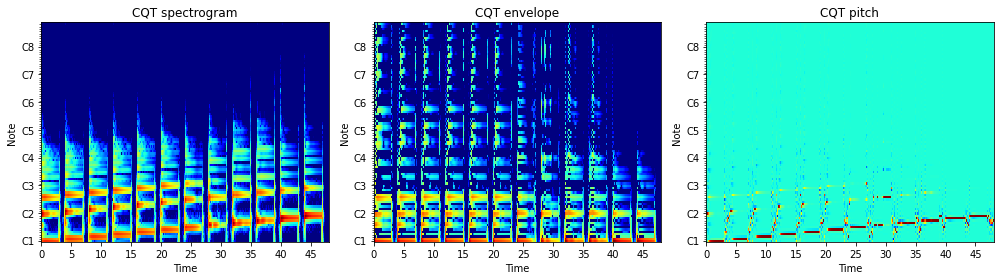
\includegraphics[width=\textwidth]{deconvolution.png}
    \caption{Deconvolution of the CQT-spectrogram (left plot, shown in dB) of 12 acoustic bass notes playing from C1 to B1, into a pitch-independent spectral envelope (middle plot, shown in dB) and an energy-normalized pitch component (right plot, shown in $[0, 1]$).}
    \label{fig:deconvolution}
\end{figure*}

This deconvolution process can also be thought of as the normalization of the log-spectrum by the magnitude of its FT (which here would correspond to the FT of the envelope) leading to a sharper log-spectrum (which here would correspond to the pitch component), in the manner of the generalized cross-correlation phase transform (GCC-PHAT) method which aims at normalizing a cross-correlation function by its magnitude spectrum to sharpen the cross-correlation peaks \cite{knapp1976}.


\subsection{Extraction of the spectral envelope coefficients}

Once the CQT-spectrum has been decomposed into an envelope and a pitch component, we can then assume that most of the pitch information has been removed from the envelope which now mostly contains the timbre information. As shown in the middle plot of Figure \ref{fig:deconvolution}, the envelope can be thought of as a pitch-normalized log-spectrum where the spectral components, in particular, the harmonics which contain most of the energy of the musical instrument, have been essentially brought down to the same note level. Given the octave resolution that was used to compute the CQT-spectrum, i.e., the number of bins per octave, we can then easily infer the locations of those harmonics in the envelope. We can subsequently extract these harmonics, or \textit{spectral envelope coefficients}, from the envelope, and therefore obtain a compact and meaningful feature for characterizing the timbre of the musical instrument. Equation \ref{eq:extraction} shows how to derive the indices of the spectral envelope coefficients given $O_r$, the octave resolution, and $N_c$, the number of desired coefficients, and consequently extract the CQT-SECs from the envelope $E$, with $\log_2(.)$ and $round(.)$ representing the binary logarithm and the round function, respectively.
\begin{equation}
\label{eq:extraction}
\begin{split}
\begin{cases}
i = round(O_r \log_2(k)) \\
\text{CQT-SEC}_k = E(i) \\
\end{cases}
\quad 1 \le k \le N_c
\end{split}
\end{equation}

Figure \ref{fig:extraction} shows an example of CQT-SECs ...

in dB

\begin{figure*}[htp]
    \centering
    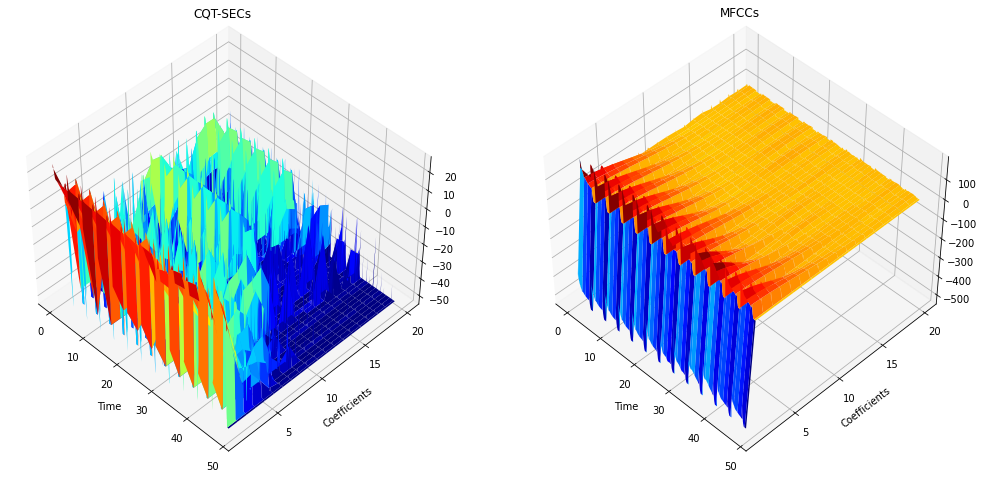
\includegraphics[width=\textwidth]{extraction.png}
    \caption{Example of CQT-SECs ... (left plot, shown in dB), and MFCCs ... (right plot).}
    \label{fig:extraction}
\end{figure*}

We recall how the MFCCs are computed ...\cite{mermelstein1976}
mel scale: \cite{stevens1937}



\section{Numerical Examples} % or "V - Computational Example"

\subsection{Analysis on an Example}

%- The envelope component can additionally be refined, along with the pitch component


\subsection{Comparison on a Dataset}


%Figure \ref{fig:dft_kernels} shows ...

%\begin{figure}[htbp]
%	\centering
%	\includegraphics[width=\columnwidth]{dft_kernels.png}
%	\caption{Kernels derived from the Hanning (top-left), Blackman (top-right), triangular (center-left), Parzen (center-right), Gaussian (with $\alpha = 2.5$) (bottom-left), and Kaiser (with $\beta = 0.5$) (bottom-right) windows. The kernels were derived for an $N$-point DFT where $N = 2048$ samples. Only the first 100 coefficients at the bottom-left corner of the $N$-by-$N$ kernels are shown. The values are displayed in log of amplitude.}
%	\label{fig:dft_kernels}
%\end{figure}


\section{What We Have Learned}

We have shown that we can derive a simple but function timbre feature which is more adapted to musical data ...

%Limitations:
%- just like MFCCs, not very robust to noise, to mixture of musical instruments playing at different pitches



\section{Author}

\textit{\textbf{Zafar Rafii}} (zafarrafii@gmail.com) received a PhD in Electrical Engineering and Computer Science from Northwestern University in 2014, and an MS in Electrical Engineering from both Ecole Nationale Superieure de l’Electronique et de ses Applications in France and Illinois Institute of Technology in the US in 2006. He is currently a senior research engineer at Gracenote in the US. He also worked as a research engineer at Audionamix in France. His research interests are centered on audio analysis, somewhere between signal processing, machine learning, and cognitive science, with a predilection for source separation and audio identification.

\bibliographystyle{IEEEtran}
\bibliography{bibliography.bib}

\end{document}
